\documentclass[11pt,class=report,crop=false]{standalone}
\usepackage[screen]{../python}


\begin{document}


%====================================================================
\chapitre{Mouvement de particules}
%====================================================================

\index{particule}

\objectifs{Tu vas simuler le mouvement d'une particule soumise à différentes forces, comme la gravité ou des frottements. Tu appliqueras ceci afin de simuler le mouvement des planètes autour du Soleil. Cette activité utilise la programmation objet.}


%%%%%%%%%%%%%%%%%%%%%%%%%%%%%%%%%%%%%%%%%%%%%%%%%%%%%%%%%%%%%%%%
%%%%%%%%%%%%%%%%%%%%%%%%%%%%%%%%%%%%%%%%%%%%%%%%%%%%%%%%%%%%%%%%

\begin{cours}[Une particule]

\textbf{Modélisation.}
Une particule est modélisée par cinq valeurs :
\begin{itemize}
  \item ses coordonnées $x$ et $y$,
  \item les coordonnées $v_x$ et $v_y$ de sa vitesse,
  \item sa masse $m$.
\end{itemize}

  \myfigure{1}{
\tikzinput{fig-particule-0}
}

\textbf{Particule soumise à aucune force.}
Si aucune force n'agit sur la particule, alors elle conserve sa direction et sa vitesse. Ainsi à l'instant élémentaire suivant, la nouvelle position de la particule est :
$$\left\lbrace
\begin{array}{rcl}
x' &=& x + v_x \\
y' &=& y + v_y \\
\end{array}
\right.$$
La particule a donc un mouvement rectiligne uniforme.

\emph{Preuve.}
La vitesse est la dérivée de la position, ainsi par exemple
$v_x$ est la limite du taux d'accroissement $\frac{x(t+\dd t)-x(t)}{\dd t}$.
En considérant que $\dd t$ est un durée infinitésimale on obtient ;
$x(t+\dd t) = x(t) + v_x \dd t$. En choisissant comme unité de temps $\dd t=1$, on obtient la formule voulue. Les calculs sont identiques pour $v_y$.

\textbf{Particule soumise à une force.}
Si la particule est soumise à une force $\vec F$ dont les composantes sont 
$(F_x,F_y)$ alors à l'instant élémentaire suivant, la nouvelle \textbf{vitesse}
de la particule est :
$$\left\lbrace
\begin{array}{rcl}
v_x' &=& v_x + F_x/m \\
v_y' &=& v_y + F_y/m \\
\end{array}
\right.$$
Comme la vitesse est modifiée, cela induit un changement sur la future position. 

\emph{Preuve.}
Le principe fondamental de la mécanique affirme que :
$$\vec F = m \vec a$$
où $\vec a$ est le vecteur accélération et $m$ la masse. L’accélération est la dérivée de la vitesse, donc en coordonnées on a :
$$F_x = m \frac{\dd v_x}{\dd t} \qquad  F_y = m \frac{\dd v_y}{\dd t}$$
Autrement dit $m\frac{v_x(t+\dd t) - v_x(t)}{\dd t} = F_x$.
Donc $v_x(t+\dd t) = v_x(t) + \frac{F_x}{m} \dd t$. En normalisant à $\dd t=1$, on obtient la formule voulue.
  
  
\medskip
S'il y a plusieurs forces $\vec F_1$, $\vec F_2$\ldots{} alors on les regroupe en un seul vecteur, la force résultante : $\vec F = \vec F_1 + \vec F_2 + \cdots$
\end{cours}



%%%%%%%%%%%%%%%%%%%%%%%%%%%%%%%%%%%%%%%%%%%%%%%%%%%%%%%%%%%%%%%%
% Activité 1 - 
%%%%%%%%%%%%%%%%%%%%%%%%%%%%%%%%%%%%%%%%%%%%%%%%%%%%%%%%%%%%%%%%

\begin{activite}[Une particule]

\objectifs{Objectifs : programmer le mouvement d'une particule et son affichage.}


Informatiquement, on code une particule par un objet de la classe \ci{Particule()} contenant $5$ attributs \ci{x}, \ci{y}, \ci{vx}, \ci{vy}, \ci{m} (correspondant à $x$, $y$, $v_x$, $v_y$, $m$). Voici le début de la définition de la classe \ci{Particule()} que tu vas peu à peu compléter :

\begin{lstlisting}
class Particule():
    def __init__(self,x,y,vx,vy,m):
        self.x = x
        self.y = y
        self.vx = vx
        self.vy = vy
        self.m = m

    def __str__(self):
        ligne = "("+str(self.x)+","+str(self.y)+"),
        ("+str(self.vx)+", "+str(self.vy)+"), "+str(self.m)
        return ligne 
\end{lstlisting}

Voici un exemple d'initialisation d'une particule \ci{p} placée en $(-100,100)$ avec une vitesse de vecteur $(20,0)$ (donc horizontale) et de masse $m=1$. La méthode \ci{__str__()} définie plus haut permet d'afficher proprement l'objet \ci{p}.
\begin{lstlisting}
p = Particule(-100,100,20,0,1)
print(p)
\end{lstlisting}

\begin{enumerate}
  \item Complète la définition de la classe avec une méthode \ci{action_vitesse(self)} qui déplace la particule en suivant le vecteur vitesse. Les nouvelles coordonnées sont données par la formule :
  
\begin{minipage}{0.4\textwidth}
  $$\left\lbrace\begin{array}{rcl}x' &=& x+ v_x\\y'&=&y+v_y\end{array}\right.$$
\end{minipage}
\begin{minipage}{0.49\textwidth}  
  \myfigure{1}{
\tikzinput{fig-particule-1}
}
\end{minipage}

  \item Complète la définition de la classe avec une méthode \ci{affiche(self)} qui affiche
  graphiquement la particule.
  
  Sur la figure ci-dessous en haut à gauche une particule avec son vecteur vitesse, en haut à droite une particule sans affichage de son vecteur vitesse mais de masse plus grosse. En bas une particule qui se déplace suivant son vecteur vitesse (sur $10$ unités de temps, en suivant un mouvement rectiligne uniforme).
  
\begin{center}
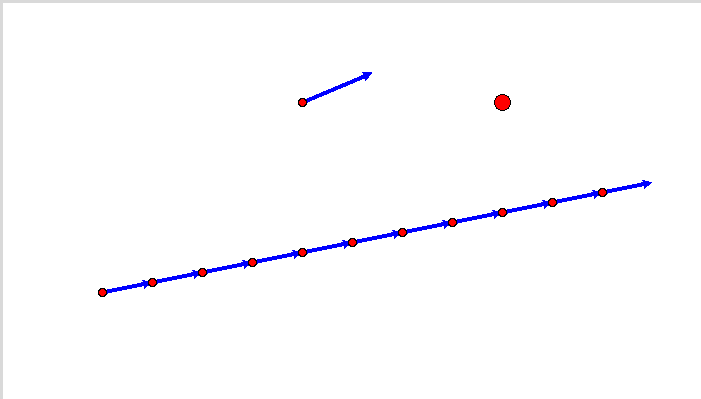
\includegraphics[scale=\myscale,scale=0.4]{ecran-particule-1}
\end{center}	 

\emph{Indications.}
\begin{itemize}
  \item Utilise le module \ci{tkinter} (voir plus bas) (avec une unité qui vaut un pixel, le point $(0,0)$ étant au centre de l'écran). Le passage des coordonnées réelles aux coordonnées graphiques se fait par les formules   \ci{i = Largeur//2 + x} \  et \   \ci{j = Hauteur//2 - y}.
  \item Tu peux définir ta fonction avec une entête \ci{affiche(self,avec_fleche=False)} et laisser le choix de l'affichage du vecteur vitesse sous la forme d'une flèche.
  \item Le rayon du disque peut dépendre de la masse.
  \end{itemize}
  
  
  
  
  \item Complète la définition de la classe avec une méthode \ci{action_gravite(self,gravite=0.2)} qui correspond à l'action de la force de gravité sur la particule. Cela correspond à changer la valeur de la vitesse verticale, la nouvelle valeur $v_y'$ étant calculée à partir de l'ancienne valeur $v_y$ par la formule :
  $$v_y' = v_y - g.$$
  Teste différentes valeurs de la constante de gravité.
  
\begin{center}
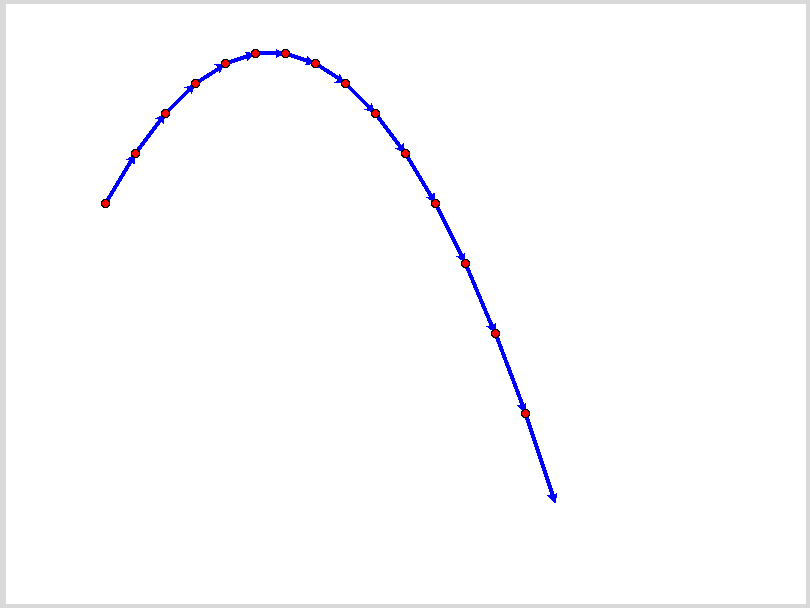
\includegraphics[scale=\myscale,scale=0.25]{ecran-particule-2}\qquad
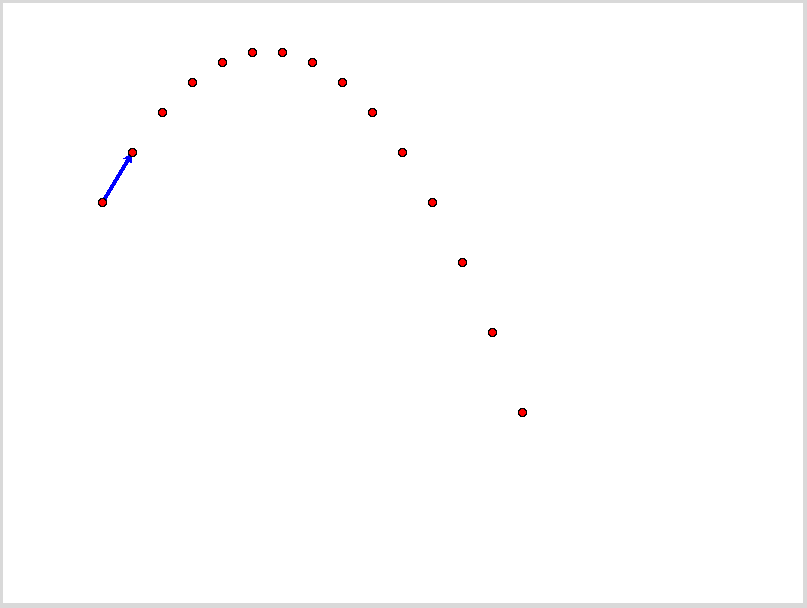
\includegraphics[scale=\myscale,scale=0.25]{ecran-particule-3}
\end{center}	 

   Comme on peut le voir sur les formules (et sur les tracés) il est remarquables que les mouvements de particules de deux masses différentes sont identiques.
   
  \item Complète la définition de la classe avec une méthode \ci{rebondir_si_bord_atteint(self)} qui empêche la particule de sortir de l'écran. Pour cela si $x$ est trop grand ou trop petit alors inverse le signe de $v_x$ (c'est-à-dire \ci{vx} $\leftarrow$ \ci{-vx}). De même pour $y$.
 
\begin{center}
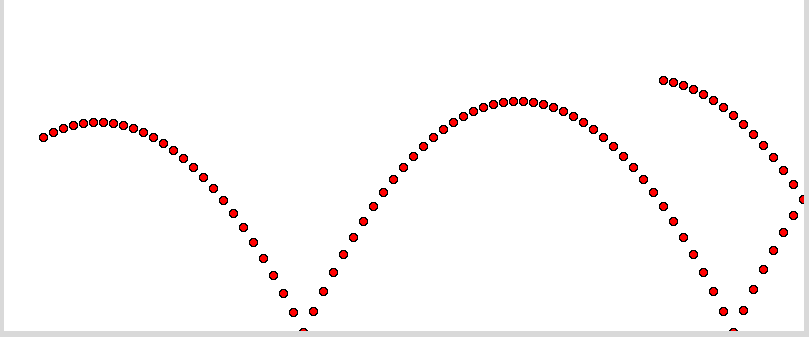
\includegraphics[scale=\myscale,scale=0.4]{ecran-particule-4}
\end{center}	  

  \item Complète la définition de la classe avec une méthode
   \mycenterline{\ci{action_frottement(self,frottement=0.005,exposant=2)}}
  qui correspond à l'action d'une force de frottement.
  
  
  On note 
  $$v = \sqrt{v_x^2 + v_y^2}.$$
  Les nouvelles valeurs du vecteur vitesse sont données par les formules :
  $$  \left\lbrace\begin{array}{rcl}
  v_x' &=& v_x - \dfrac{f}{m} \cdot v^e \cdot \dfrac{v_x}{v}\\[1em]
  v_y' &=& v_y - \dfrac{f}{m} \cdot v^e \cdot \dfrac{v_y}{v}
  \end{array}\right.$$
  où $f$ est le coefficient de frottement et $e$ l'exposant de frottement.
  Essaie différentes valeurs du coefficient de frottement et surtout de l'exposant. Un exposant $e=1$ correspond à un frottement pour une particule se déplaçant à faible vitesse ; un exposant $e=2$ correspond à une vitesse élevée ; des exposants $1<e<2$ sont possibles.

\begin{center}
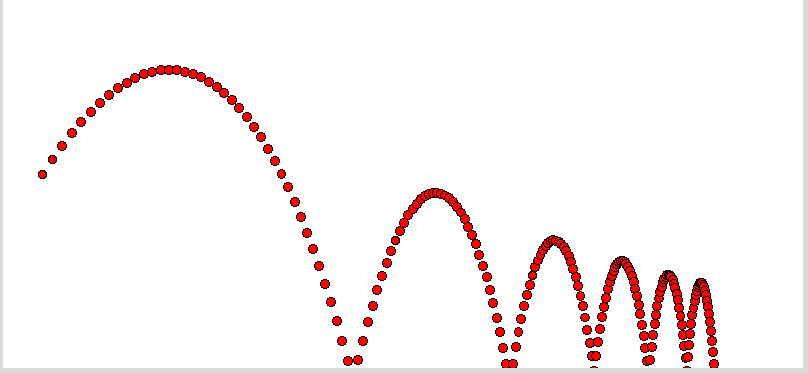
\includegraphics[scale=\myscale,scale=0.41]{ecran-particule-5}
\end{center}	  
  
   
  \item Complète la définition de la classe avec une méthode \ci{mouvement(self)} qui regroupe la succession des actions définies : \ci{action_vitesse()}, \ci{action_gravite()}, \ci{action_frottement()}, \ci{rebondir_si_bord_atteint()} Ainsi pour simuler le mouvement d'une particule il suffit d'écrire :\index{module!tkinter@\ci{tkinter}} 
  
\begin{lstlisting}
# Constantes pour l'affichage
Largeur = 800
Hauteur = 600

# Fenêtre tkinter
from tkinter import *

root = Tk()      
canvas = Canvas(root, width=Largeur, height=Hauteur, background="white")
canvas.pack(side=LEFT, padx=5, pady=5)

p = Particule(-300,10,5,2,10)
for k in range(100):
    p.mouvement()
    p.affiche()
    
root.mainloop()
\end{lstlisting} 

\end{enumerate} 

\end{activite}




%%%%%%%%%%%%%%%%%%%%%%%%%%%%%%%%%%%%%%%%%%%%%%%%%%%%%%%%%%%%%%%%
% Activité 2 - Une particule en mouvement
%%%%%%%%%%%%%%%%%%%%%%%%%%%%%%%%%%%%%%%%%%%%%%%%%%%%%%%%%%%%%%%%

\begin{activite}[Particules en mouvement]

\objectifs{Objectifs : afficher une ou plusieurs particules en mouvement.}

Voici le \og{}film\fg{} de $10$ particules, chacune étant lancée à partir du même point mais avec un vecteur vitesse initial différent.

\begin{center}
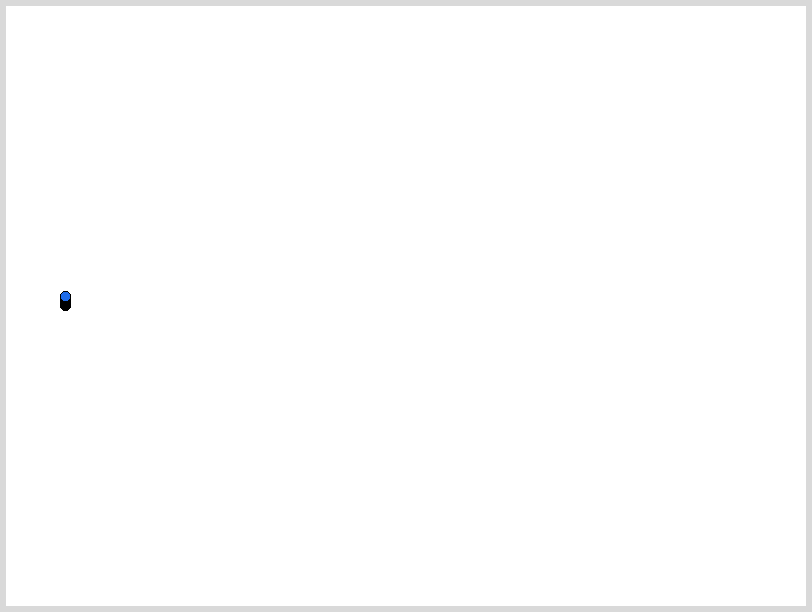
\includegraphics[scale=\myscale,scale=0.18]{ecran-mouvement-001}\ 
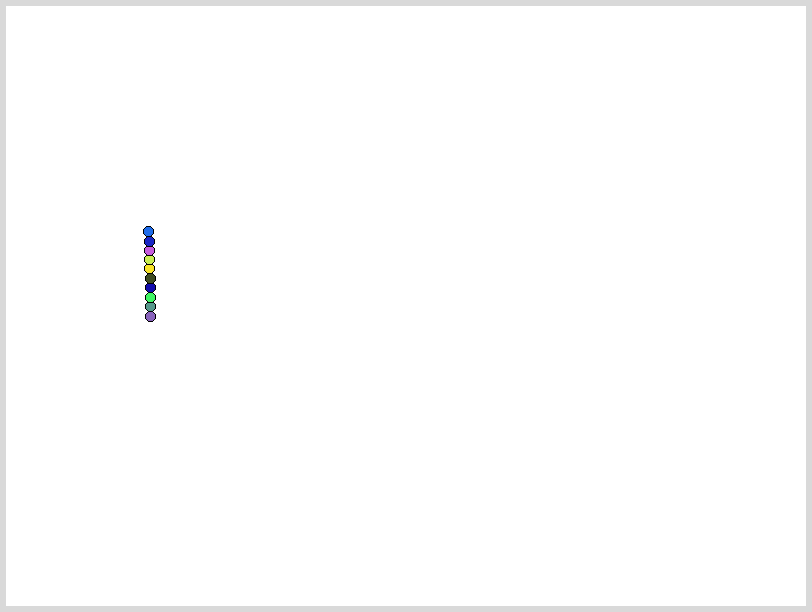
\includegraphics[scale=\myscale,scale=0.18]{ecran-mouvement-010}\ 
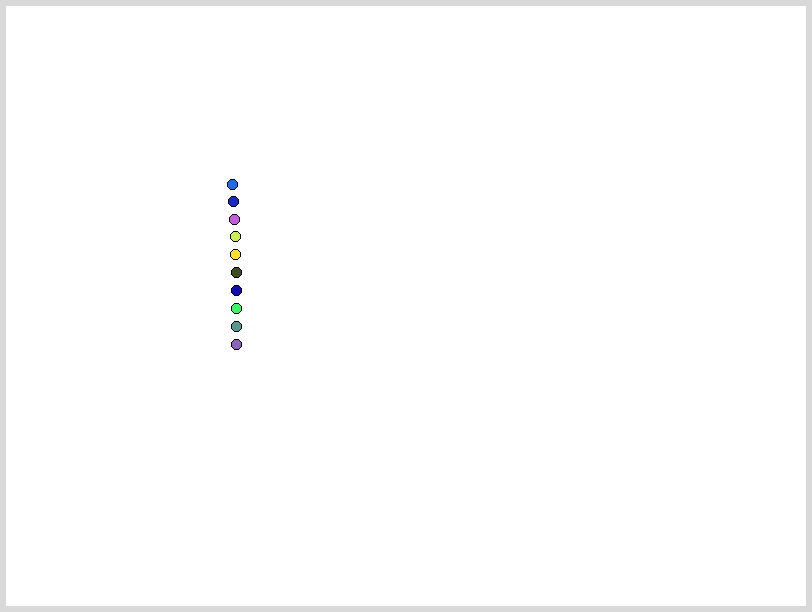
\includegraphics[scale=\myscale,scale=0.18]{ecran-mouvement-020}

\smallskip

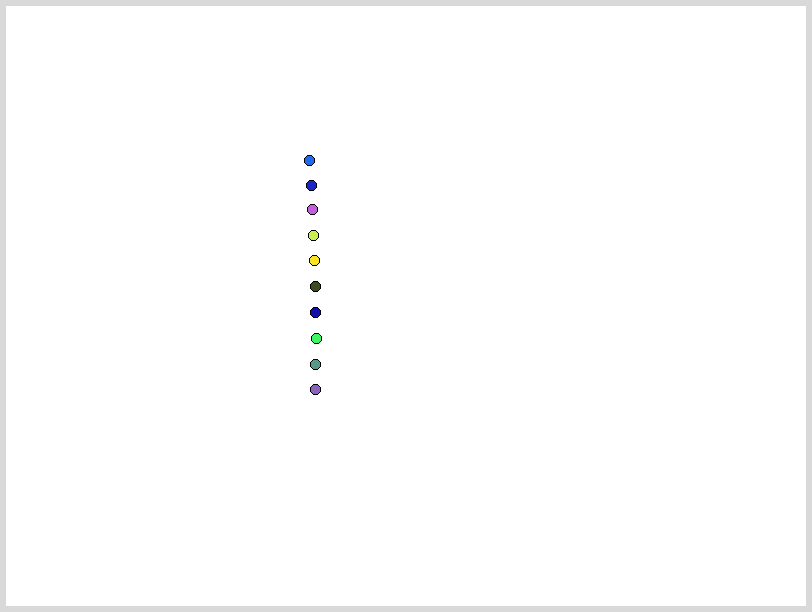
\includegraphics[scale=\myscale,scale=0.18]{ecran-mouvement-030}\ 
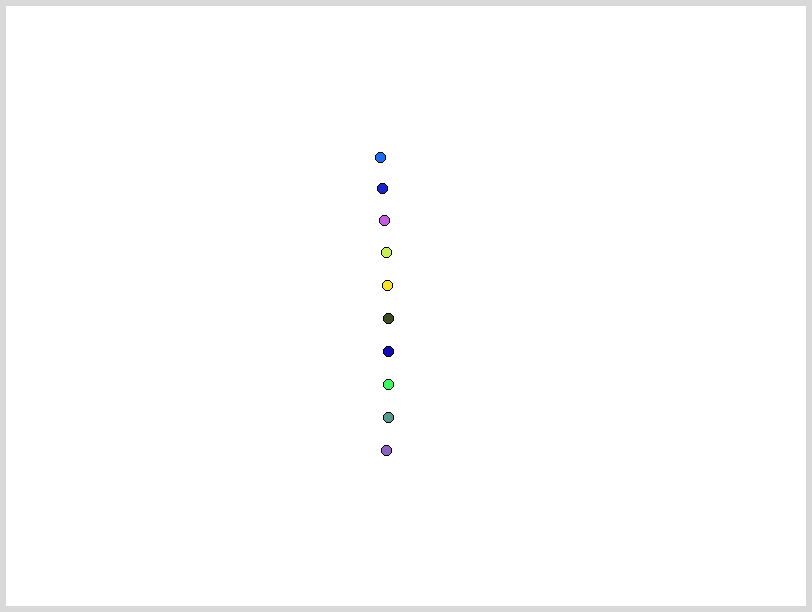
\includegraphics[scale=\myscale,scale=0.18]{ecran-mouvement-040}\ 
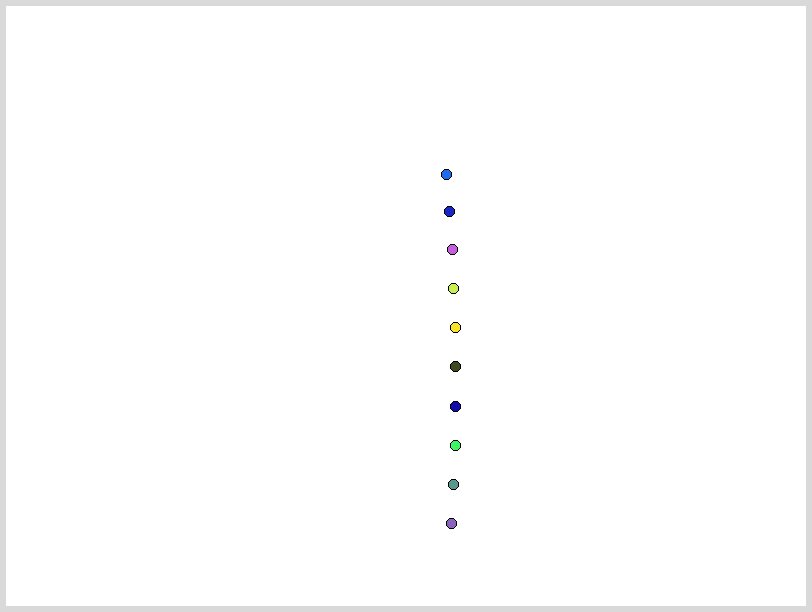
\includegraphics[scale=\myscale,scale=0.18]{ecran-mouvement-050}
\end{center}	 

Programme tout cela en utilisant les explications qui suivent.

\bigskip

Voici une classe \ci{TkParticule()} héritée de la classe \ci{Particule()} qui
permet d'afficher une particule en mouvement (la particule évolue sans afficher sa trace). 
Il y a deux attributs supplémentaires :
un attribut pour la couleur, un attribut pour l'identifiant \ci{tkinter} de la particule qui permet ensuite à la méthode \ci{affiche()} de déplacer le disque grâce à la méthode \ci{move()} de \ci{tkinter}.

\begin{lstlisting}
class TkParticule(Particule):
    def __init__(self,x,y,vx,vy,m,couleur="red"):
        Particule.__init__(self,x,y,vx,vy,m)
        self.couleur = couleur
        i,j = xy_vers_ij(x,y)
        rayon = min(max(1,m),10)
        # Création de l'objet tkinter
        disque = canvas.create_oval(i-rayon,j-rayon,
                 i+rayon,j+rayon,fill=self.couleur)
        self.id = disque

    def affiche(self):
        canvas.move(self.id,self.vx,-self.vy)
\end{lstlisting}

La fonction \ci{xy_vers_ij(x,y)} transforme les coordonnées réelles $(x,y)$ en coordonnées graphiques $(i,j)$.


Voici un lancé de plusieurs particules (on utilise le module \ci{time}).
\begin{lstlisting}
liste_particules = [TkParticule(-300,0,10,j,5,couleur=hasard_couleur()) 
                    for j in range(10)]
for k in range(200):
    for p in liste_particules:
        p.mouvement()
        p.affiche()

    canvas.update()
    sleep(0.05)

root.mainloop()
\end{lstlisting}


Voici une fonction qui renvoie une couleur au hasard (en utilisant le module \ci{random}).
\begin{lstlisting}
def hasard_couleur():
    R,V,B = randint(0,255),randint(0,255),randint(0,255)
    couleur = '#%02x%02x%02x' % (R%256, V%256, B%256)
    return couleur
\end{lstlisting}


Une autre idée est de garder la trace des positions précédentes.
\begin{center}
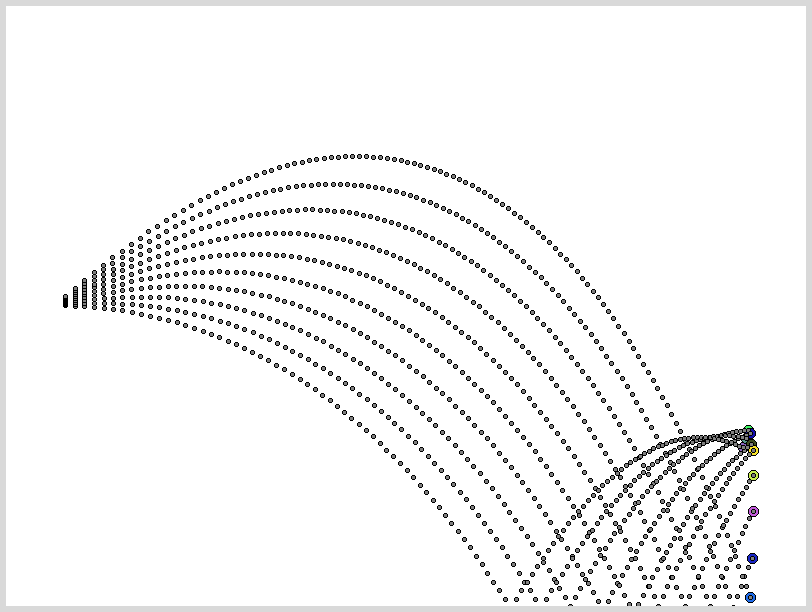
\includegraphics[scale=\myscale,scale=0.4]{ecran-mouvement-trace}
\end{center}	 

\end{activite}



%%%%%%%%%%%%%%%%%%%%%%%%%%%%%%%%%%%%%%%%%%%%%%%%%%%%%%%%%%%%%%%%
%%%%%%%%%%%%%%%%%%%%%%%%%%%%%%%%%%%%%%%%%%%%%%%%%%%%%%%%%%%%%%%%

\begin{cours}[Attraction gravitationnelle]

Deux astres s'attirent selon la force d'attraction gravitationnelle :

\begin{minipage}{0.4\textwidth}  
$$\vec G = G \frac{m_1 m_2}{r^2} \vec u$$
\end{minipage}
\begin{minipage}{0.4\textwidth}  
  \myfigure{1}{
\tikzinput{fig-particule-2}
}
\end{minipage}

où
\begin{itemize}
  \item les astres sont de masses $m_1$ et $m_2$,
  \item $r$ est la distance entre les deux astres,
  \item $G$ est la constante de gravitation universelle (on prendra arbitrairement $G=100$),
  \item et $\vec u$ est un vecteur unité pointant de l'astre 1 vers l'astre 2.
\end{itemize}

Avec ces notations $\vec G$ est la force d'attraction de l'astre 2 agissant sur l'astre 1,
et $-\vec G$ est la force d'attraction de l'astre 1 agissant sur l'astre 2. 

On note $(x_1,y_1)$, $(x_2,y_2)$ les coordonnées des astres.
On pose :
$$x = x_2-x_1 \qquad  y = y_2-y_1 \qquad r = \sqrt{x^2+y^2}$$
Les coordonnées du vecteur $\vec G$ sont alors :
$$g_x = G \frac{m_1 m_2}{r^2} \cdot \frac{x}{r} 
\quad \text{ et } \quad
g_y = G \frac{m_1 m_2}{r^2} \cdot \frac{y}{r}$$  
  \myfigure{1}{
\tikzinput{fig-particule-3}
}

\end{cours}



%%%%%%%%%%%%%%%%%%%%%%%%%%%%%%%%%%%%%%%%%%%%%%%%%%%%%%%%%%%%%%%%
% Activité 3 - Mouvement des planètes
%%%%%%%%%%%%%%%%%%%%%%%%%%%%%%%%%%%%%%%%%%%%%%%%%%%%%%%%%%%%%%%%

\begin{activite}[Mouvement des planètes]

\objectifs{Objectifs : simuler le mouvement des planètes autour du Soleil grâce à la force de gravitation.}

\begin{center}
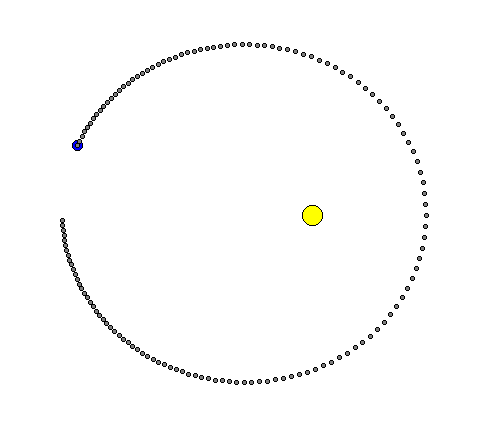
\includegraphics[scale=\myscale,scale=0.4]{ecran-planetes-1}
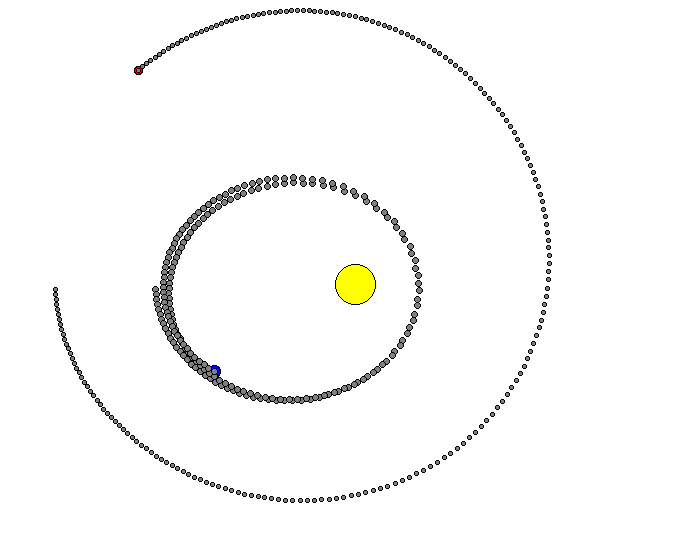
\includegraphics[scale=\myscale,scale=0.3]{ecran-planetes-3}
\end{center}	
Figure de gauche : la Terre\couleurnb{ (en bleu)}{} et le Soleil. Le Soleil est fixe. La Terre parcourt une orbite elliptique. Note que lorsqu'elle se rapproche du Soleil la Terre va plus vite.

Figure de droite : Mars (\couleurnb{en rouge }{}à l'extérieur), la Terre\couleurnb{ (en bleu)}{} et le Soleil. Note que le mouvement de la Terre est perturbé par Mars.
Dans la réalité le mouvement de la Terre est une ellipse quasiment circulaire et Mars influe peu sur le mouvement de la Terre (car sa masse est considérablement plus faible que celle du Soleil).

On peut aussi tracer la trajectoire d'une comète, ayant une vitesse initiale importante, qui passerait une unique fois près du Soleil avant de s'éloigner définitivement. Elle suit une trajectoire hyperbolique (figure ci-dessous).
\begin{center}
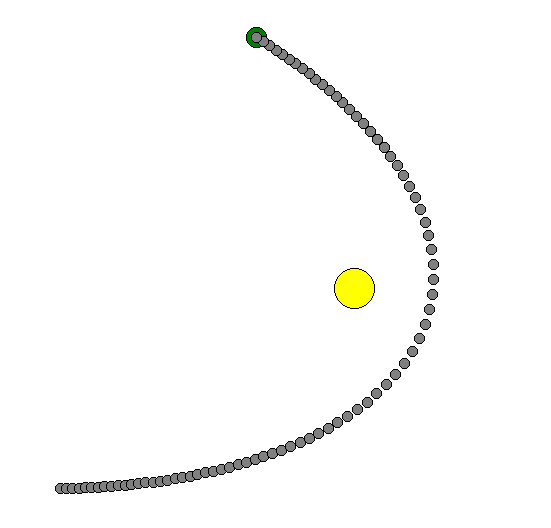
\includegraphics[scale=\myscale,scale=0.3]{ecran-planetes-4}
\end{center}	

Travail à faire :
\begin{enumerate}
  \item Programme une classe \ci{Planete} héritée de la classe \ci{Particule}.
  Cette classe contient deux méthodes: 
  \begin{itemize}
    \item une méthode \ci{action_attraction(self,other)} qui calcule la force d'attraction $(g_x,g_y)$ entre l'astre courant (l'objet \ci{self}) et un autre astre (l'objet \ci{other}) et qui modifie la vitesse de l'astre courant (de masse $m_1$) selon la formule :
  $$  \left\lbrace\begin{array}{rcl}
  v_x' &=& v_x + \dfrac{g_x}{m_1}\\[1em]
  v_y' &=& v_y + \dfrac{g_y}{m_1}
  \end{array}\right.$$  
  
    \item une méthode \ci{mouvement(self)} qui ne fait appel qu'à la méthode   \ci{action_vitesse()}.
  \end{itemize}
  
  \item Programme une classe \ci{TkPlanete} héritée de la classe \ci{Planete} (de la même façon que \ci{TkParticule()} était héritée de la classe \ci{Particule()}) avec une méthode \ci{affiche()} qui réalise l'affichage graphique avec \ci{tkinter}.
 
 
 \item Utilise ton programme pour tracer les orbites de planètes. Par exemple avec trois astres (Soleil, Terre, Mars), à chaque pas il faut calculer l'attraction entre la Terre et le Soleil, l'attraction entre la Terre et Mars, puis déplacer la Terre. Ensuite il faut faire la même chose avec Mars. On considère que le Soleil est fixe.
 
 Voici des exemples de paramètres utilisés (avec en plus $G=100$).
 \begin{lstlisting}
# Trois astres : Soleil, Terre et Mars
soleil = TkPlanete(0,0,0,0,100,"yellow")
terre = TkPlanete(-200,0,0,-5,3,"blue")
mars = TkPlanete(-300,0,0,-5,2,"red")

for k in range(200):
    terre.action_attraction(soleil)
    terre.action_attraction(mars)
    terre.mouvement()
    terre.affiche(avec_trace=True)
    mars.action_attraction(soleil)
    mars.action_attraction(terre)
    mars.mouvement()
    mars.affiche(avec_trace=True)
    
    canvas.update()
    sleep(0.02)
\end{lstlisting}
 
\end{enumerate} 

\end{activite}


\end{document}
